\documentclass[12pt]{standalone}                                                      
\usepackage{graphicx}                                                           
\usepackage{tikz}
\usepackage{varwidth}
\usetikzlibrary{calc,arrows,positioning}

\begin{document}

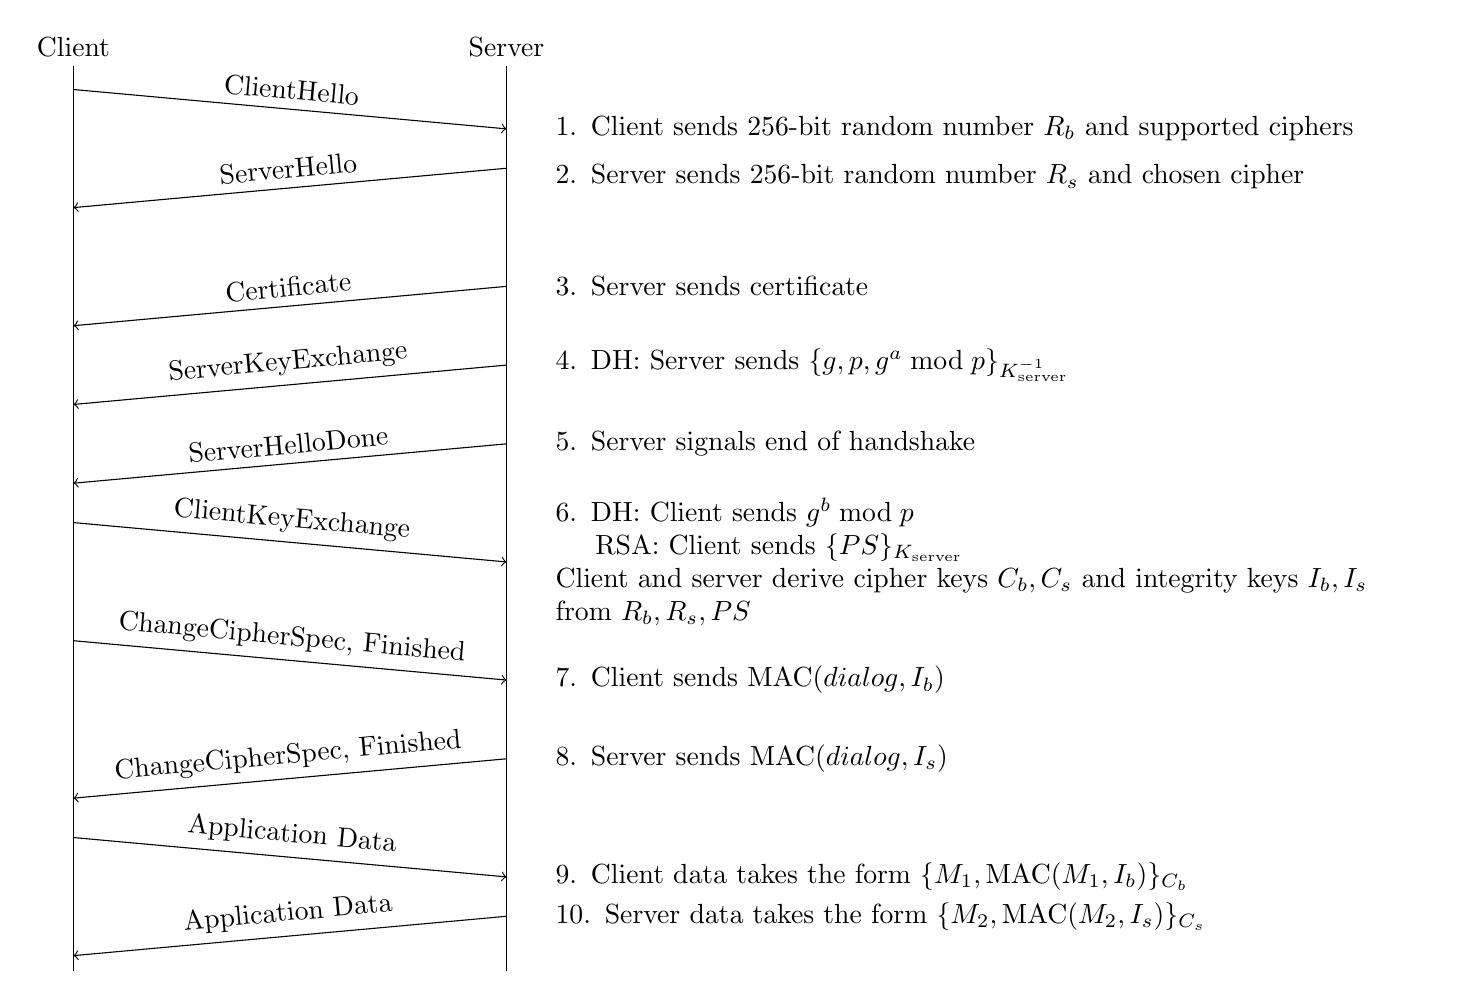
\begin{tikzpicture}
\tikzstyle{block} = [text width=11cm]
    \coordinate (ClientTop) at (0,0);                                           
    \coordinate (ServerTop) at (5.5,0);                                                                                    
    \coordinate[label=Client] (ClientBottom) at (0,11.5);                                         
    \coordinate[label=Server] (ServerBottom) at (5.5,11.5);      
    \coordinate[below=.3cm of ClientBottom] (A);
    \coordinate[below=.8cm of ServerBottom] (B);
    \node[block,right=.5cm of B] (1) {1. Client sends 256-bit random number $R_b$ and supported ciphers};
    \coordinate[below=.5cm of B] (C);
    \node[block,below=.05cm of 1] (2) {2. Server sends 256-bit random number $R_s$ and chosen cipher};
    \coordinate[below=1.5cm of A] (D);
    \coordinate[below=1.5cm of C] (E);
    \node[block,right=.5cm of E] (3) {3. Server sends certificate};
    \coordinate[below=1.5cm of D] (F);
    \coordinate[below=1cm of E] (G);
    \node[block,right=.5cm of G] (4) {4. DH: Server sends $\{g, p, g^a \bmod{p} \}_{K^{-1}_\mathrm{server}}$};
    \coordinate[below=1cm of F] (H);
    \coordinate[below=1cm of G] (I);
    \node[block,right=.5cm of I] (5) {5. Server signals end of handshake};
    \coordinate[below=1cm of H] (J); 
    \coordinate[below=.5cm of J] (K);
    \coordinate[below=1.5cm of I] (L);
    \node[block,right=.5cm of L] (6) {6. DH: Client sends $g^b \bmod{p}$ \\ \hspace{11pt} RSA: Client sends $\{PS\}_{K_\mathrm{server}}$ \\ Client and server derive cipher keys $C_b, C_s$ and integrity keys $I_b, I_s$ from $R_b, R_s, PS$};
    \coordinate[below=1.5cm of K] (M);
    \coordinate[below=1.5cm of L] (N);
    \node[block,right=.5cm of N] (7) {7. Client sends MAC($dialog, I_b$)};
    \coordinate[below=1cm of N] (O);
    \coordinate[below=2cm of M] (P);
    \node[block,right=.5cm of O] (8) {8. Server sends MAC($dialog, I_s$)};
    \coordinate[below=.5cm of P] (Q);
    \coordinate[below=1.5cm of O] (R);
    \node[block,right=.5cm of R] (9) {9. Client data takes the form $\{M_1, \mathrm{MAC}(M_1, I_b)\}_{C_b}$};
    \coordinate[below=.5cm of R] (S);
    \coordinate[below=1.5cm of Q] (T);
    \node[block,right=.5cm of S] (10) {10. Server data takes the form $\{M_2, \mathrm{MAC}(M_2, I_s)\}_{C_s}$};

    \draw (ClientTop)--(ClientBottom);                                          
    \draw (ServerTop)--(ServerBottom);           
    \draw[->] (A) -- (B)  node[midway,sloped,above] {ClientHello};
    \draw[->] (C) -- (D)  node[midway,sloped,above] {ServerHello};
    \draw[->] (E) -- (F)  node[midway,sloped,above] {Certificate};
    \draw[->] (G) -- (H)  node[midway,sloped,above] {ServerKeyExchange};
    \draw[->] (I) -- (J)  node[midway,sloped,above] {ServerHelloDone};
    \draw[->] (K) -- (L)  node[midway,sloped,above] {ClientKeyExchange};
    \draw[->] (M) -- (N)  node[midway,sloped,above] {ChangeCipherSpec, Finished};
    \draw[->] (O) -- (P)  node[midway,sloped,above] {ChangeCipherSpec, Finished};
    \draw[->] (Q) -- (R)  node[midway,sloped,above] {Application Data};
    \draw[->] (S) -- (T)  node[midway,sloped,above] {Application Data};
\end{tikzpicture}


\end{document}